\documentclass[onecolumn]{aastex63}
\usepackage{natbib}
%\definecolor{orcidlogocol}{HTML}{A6CE39}
\bibliographystyle{aasjournal}

\begin{document}

\title{PLANETESIMAL ACCRETION AT SHORT ORBITAL PERIODS}

\author{Spencer C. Wallace}
\affiliation{Astronomy Department, University of Washington, Seattle, WA 98195}


\author{Thomas R. Quinn}
\affiliation{Astronomy Department, University of Washington, Seattle, WA 98195}

\begin{abstract}
Abstract goes here
\end{abstract}

\section{Introduction} \label{sec:intro}

Intro text goes here \citep{2019MNRAS.489.2159W}

\begin{figure}
    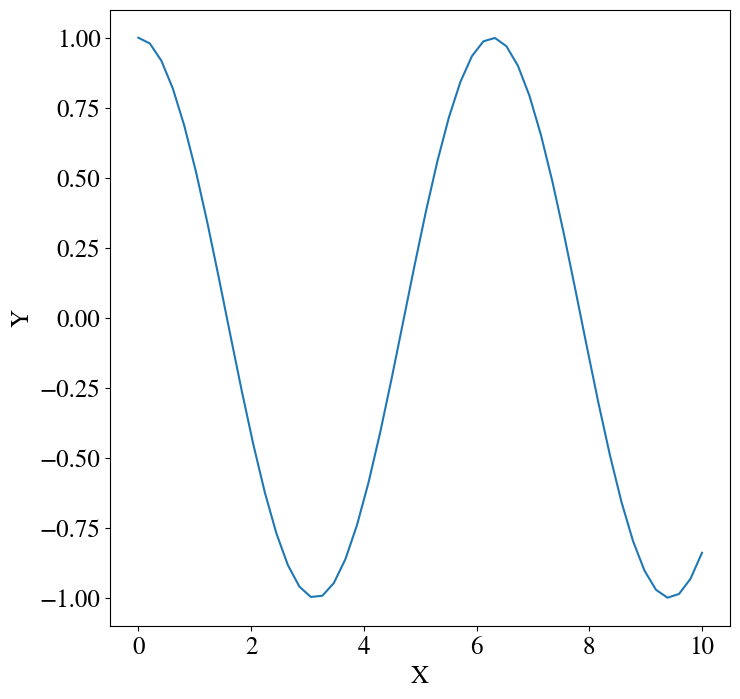
\includegraphics[width=0.5\columnwidth]{figures/test.png}
    \caption{Caption goes here.\label{fig:test}}
\end{figure}

\section{Collision and Relaxation Timescale}

The motivation for this project comes from the realization that the collision timescale and the relaxation time (which sets the timescales for things like viscous stirring and dynamical friction (cite ida 1993)) do not scale proportionately with orbital period. At sufficiently long orbital periods, the relaxation time is shorter than the collision time. This means that as planetesimals grow, the velocity distribution of bodies reacts to the changing mass distribution, which alters the growth mode. When this condition is met, oligarchic growth can commence (cite ki 1998), which keeps the planetary embryos on circular orbits and restricts their growth.

Because these two timescales scale differently with orbital period (or equivalently semimajor axis), they should eventually cross as one gets close enough to the host star. In regions where the collision timescale is shorter than the growth time, the embryos will maintain eccentric orbits as they grow, which greatly widens their feeding zones. Because they do not settle onto circular orbits, the timescale for orbital instability, which marks the beginning of the final planet-forming phase, should be much shorter.

\subsection{Collision Timescale}

The timescale for collisions is set by

\begin{equation}
	t_{coll} = \frac{1}{n \sigma v}
\end{equation}

\noindent where $n$ is the number density of planetesimals, $\sigma$ is the cross section for collisions and $v$ is the typical encounter velocity between planetesimals. 

The number density of planetesimals is set by

\begin{equation}
    n = \frac{\Sigma \Omega}{2 m v}
\end{equation}

\noindent where $\Sigma$ is the surface density of solids in the disk, $\Omega$ is the orbital frequency and $m$ is the mass of a planetesimal. For our purposes, we will assume that the surface density profile follows a power law such that $\Sigma = A r^{-\alpha}$. Planetesimals are typically large enough to exert a significant gravitational pull on each other, which enhances the collision cross section beyond its geometric value

\begin{equation}
	\sigma = \pi s^{2} \left( 1 + \frac{v_{esc}^{2}}{v^{2}} \right)
\end{equation}

\noindent where $s$ is the radius of a planetesimal and $v_{esc}$ is the escape velocity from the surface of a planetesimal. Finally, $v$ is given by

\begin{equation}
	v = \sqrt{\left<  e^{2} \right>^{1/2} + \left< i^{2} \right>^{1/2}} v_{k}
\end{equation}

\noindent For simplicity, we will assume that the rms eccentricity and inclination of the planetesimals does not vary with orbital distance. Putting this all together, the collision timescale scales with the orbital distance and the surface density profile parameters ($A$, $\alpha$) like

\begin{equation}
	t_{coll} \sim A^{-1} r^{\alpha + 1/2}
\end{equation}

\noindent Note that a surface density profile with $\alpha < -1$ produces a collision timescale that scales more steeply than the orbital timescale. In this case, an N-body simulation will get more computationally expensive with orbital distance because the time step size scales with the orbital timescale.

\subsection{Relaxation Timescale}

The relaxation timescale is given by (citation)

\begin{equation}
    t_{relax} = \frac{v^3}{n \pi G^{2} m^{2} \ln \lambda}
\end{equation}

\noindent where $G$ is the gravitational constant and $\ln \lambda$ is the Coulomb logarithm. Using the same assumptions as above, the relaxation time scales with orbital distance and the surface density profile parameters as

\begin{equation}
    t_{relax} \sim A^{-1} r^{\alpha - 1/2}
\end{equation}

Note that this has a different dependence on $r$ than the collision timescale. Taking the ratio of these two timescales gives

\begin{equation}
\frac{t_{relax}}{t_{coll}} \sim r^{-1}
\end{equation}

The relaxation time drops relative to the collision timescale with distance.

\section{Summary and Discussion} \label{sec:discuss}

Summary and discussion text goes here

\bibliography{references}

\clearpage

\end{document}